\documentclass[pdf]{beamer}
%\mode<presentation>{}

\usepackage{amssymb,amsmath,amsthm,enumerate}
\usepackage[utf8]{inputenc}
\usepackage{array}
\usepackage[parfill]{parskip}
\usepackage{graphicx}
\usepackage{caption}
\captionsetup[figure]{labelformat=empty}
\usepackage{subcaption}
\usepackage{bm}
\usepackage{amsfonts,amscd}
%\usepackage{gensymb}
\usepackage[]{units}
\usepackage{listings}
\usepackage{multicol}
\usepackage{tcolorbox}
\usepackage{physics}
\usepackage{multimedia} % movies!
\usepackage[export]{adjustbox} % crop graphics

\usepackage{pgfpages}
\usepackage{ifthen} % package required
\usepackage[subpreambles=true]{standalone}
\usepackage{appendixnumberbeamer}
\usepackage{rotating}

\setbeameroption{show notes on second screen}

%new commands
\newcommand{\der}[2]{\frac{d#1}{d#2}}
\newcommand{\nder}[3]{\frac{d^#1 #2}{d #3 ^ #1}}
\newcommand{\pder}[2]{\frac{\partial #1}{\partial #2}}
\newcommand{\npder}[3]{\frac{\partial ^#1 #2}{\partial #3^#1}}
\newcommand{\sentencelist}{def}
\newcommand{\overbar}[1]{\mkern 1.5mu\overline{\mkern-1.5mu#1\mkern-1.5mu}\mkern 1.5mu}
\newcommand{\lined}{\overbar}
\newcommand{\perm}[2]{{}^{#1}\!P_{#2}}
\newcommand{\comb}[2]{{}^{#1}C_{#2}}
\newcommand{\intall}{\int_{-\infty}^{\infty}}
\newcommand{\Var}[1]{\text{Var}\left(#1\right)}
\newcommand{\E}[1]{\text{E}\left(#1\right)}
\newcommand{\define}{\equiv}
\newcommand{\diff}[1]{\mathrm{d}#1}
\newcommand{\empy}[1]{{\color{darkorange}\emph{#1}}}
\newcommand{\empr}[1]{{\color{cardinalred}\emph{#1}}}


\theoremstyle{remark}
\newtheorem*{remark}{Remark}
\theoremstyle{definition}

\newcommand{\examplebox}[2]{
\begin{tcolorbox}[colframe=darkcardinal,colback=boxgray,title=#1]
#2
\end{tcolorbox}}

\newcommand{\eld}[1]{\frac{d}{dt}(\frac{\partial L}{\partial \dot #1}) - \frac{\partial L}{\partial #1}=0}
\newcommand{\euler}[1]{\frac{\partial L}{\partial #1}-\frac{d}{dt}(\frac{\partial L}{\partial \dot #1})}
\newcommand{\eulerg}[1]{\frac{\partial g}{\partial #1}-\frac{d}{dt}(\frac{\partial g}{\partial \dot #1})}
\newcommand{\divg}[1]{\nabla\cdot #1}
\newcommand{\prob}[1]{P(#1\vert I)}
\DeclareMathOperator*{\argmax}{argmax}
\DeclareMathOperator{\KL}{KL}

\beamertemplatenavigationsymbolsempty

\addtobeamertemplate{footnote}{\hskip -1.8em}{}

% ================================ %
%      Section dividers            %
\newboolean{sectiontoc}
\setboolean{sectiontoc}{true} % default to true
\AtBeginSection[]
{
  \ifthenelse{\boolean{sectiontoc}}{
    \begin{frame}<beamer>{Gliederung}
      \tableofcontents[currentsection]
    \end{frame}
  }
}

\newcommand{\sectionNoDivider}[1]{
  \setboolean{sectiontoc}{false}
  \section{#1}
  \setboolean{sectiontoc}{true}
}

% \newcommand<>{\makered}[1]{{\color#2{red}#1}}
% \renewcommand<>{\hyperlink}[2]{\only#3{\beameroriginal{\hyperlink}{#1}{#2}}}
\newcommand<>{\nakedfootnote}[1]{%
  \begingroup
  \renewcommand<>\thefootnote{}\footnote#2{#1}%
  \addtocounter{footnote}{-1}%
  \endgroup
}

\AtBeginSection[]
{
	\ifthenelse{\boolean{sectiontoc}}{
	  \begin{frame}<beamer>
	    \frametitle{\insertsectionhead}
	    \tableofcontents[currentsection,hideallsubsections]
	  \end{frame}
	}
}

\AtBeginSubsection[]
{
  \begin{frame}<beamer>
    \frametitle{Outline for \insertsectionhead}
    \tableofcontents[
        currentsection,
        currentsubsection,
        subsectionstyle=show/shaded/hide
    ]
  \end{frame}
}

\usetheme{Stanford}
\def \i  {\item}
\def \ai {\item[] \quad \arrowbullet}
\newcommand \si[1]{\item[] \quad \bulletcolor{#1}}
\def \wi {\item[] \quad $\ \phantom{\Rightarrow}\ $}
\def \bi {\begin{itemize}\item}
\def \ei {\end{itemize}}
\def \be {\begin{equation*}}
\def \ee {\end{equation*}}
\def \bie {$\displaystyle{}
\def \eie {{\ }$}}
\def \bsie {\small$\displaystyle{}
\def \esie {{\ }$}\normalsize\selectfont}
\def \bse {\small\begin{equation*}}
\def \ese {\end{equation*}\normalsize}
\def \bfe {\footnotesize\begin{equation*}}
\def \efe {\end{equation*}\normalsize}
\renewcommand \le[1] {\\ \medskip \lefteqn{\hspace{1cm}#1} \medskip}
\def \bex {\begin{example}}
\def \eex {\end{example}}
\def \bfig {\begin{figure}}
\def \efig {\end{figure}}
\def \btheo {\begin{theorem}}
\def \etheo {\end{theorem}}
\def \bc {\begin{columns}}
\def \ec {\end{columns}}
\def \btab {\begin{tabbing}}
\def \etab {\end{tabbing}\svneg\svneg}
\newcommand \col[1]{\column{#1\linewidth}}
\def\vneg  {\vspace{-5mm}}
\def\lvneg {\vspace{-10mm}}
\def\svneg {\vspace{-2mm}}
\def\tvneg {\vspace{-1mm}}
\def\vpos  {\vspace{5mm}}
\def\lvpos {\vspace{10mm}}
\def\svpos {\vspace{2mm}}
\def\tvpos {\vspace{1mm}}
\def\hneg  {\hspace{-5mm}}
\def\lhneg {\hspace{-10mm}}
\def\shneg {\hspace{-2mm}}
\def\thneg {\hspace{-1mm}}
\def\hpos  {\hspace{5mm}}
\def\lhpos {\hspace{10mm}}
\def\shpos {\hspace{2mm}}

\logo{
\includegraphics[height=0.5in]{./style_files_stanford/SU_New_BlockStree_2color.png}}



\title[\insertsectionhead]{Variational Bayesian Methods (in Neuroscience)}
% \title[PhD Qualifying Exam]{Causal models of brain dynamics}

\begin{document}



\author[Tyler Benster \& Aaron Andalman, CNJC]{
	\begin{tabular}{c}
	\Large
	Tyler Benster \& Aaron Andalman\\
    \footnotesize
    Deisseroth (Tyler \& Aaron) and Druckmann (Tyler) Labs
\end{tabular}
\vspace{-2ex}
}

\institute{
	\vspace{2ex}
	
\includegraphics[height=0.4in]{./style_files_stanford/SU_New_BlockStree_2color.png}\\
	Computational Neuroscience Journal Club\\
	Stanford University}

\date{July 10, 2019}

\begin{noheadline}
\begin{frame}\maketitle\end{frame}
\end{noheadline}

%%%%%%%%%%%%%%%%%%%% Actual start %%%%%%%%%%%%%%%%%%%%%%%%%%%%%

\begin{frame}<beamer>
    \frametitle{Roadmap}
    \tableofcontents[subsectionstyle=hide]\
\end{frame}

\newcommand{\Zero}{Introduction: Why care about the distribution of data?}
\newcommand{\One}{Problem: Analyzing high dimensional data is hard}
\newcommand{\Two}{Solution: Variational Methods}
\newcommand{\Three}{Example: variational autoencoder}

\section{\Zero}

\begin{frame}[t]{The probability distribution revolution}
	\begin{multicols}{2}
		\begin{itemize}
			\item Karl Pearson (1857-1936) came with the idea that scientific measurements should be conceived as coming from probability distributions.
			\item Scientific measurements are just random reflections of the underlying truth that is the distribution.
			\item “A great book on the
history of statistics” $\rightarrow$ Aaron
			\item
		\end{itemize}

		\columnbreak

		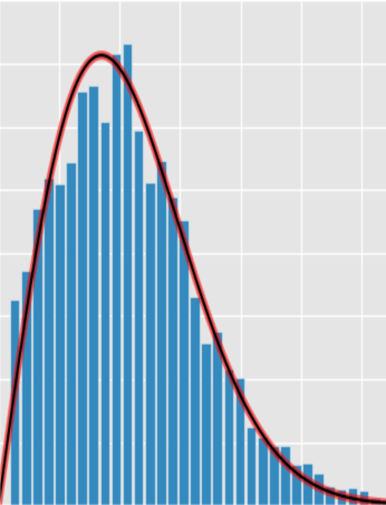
\includegraphics[width=0.25\textwidth]{media/distribution}
		\linebreak
		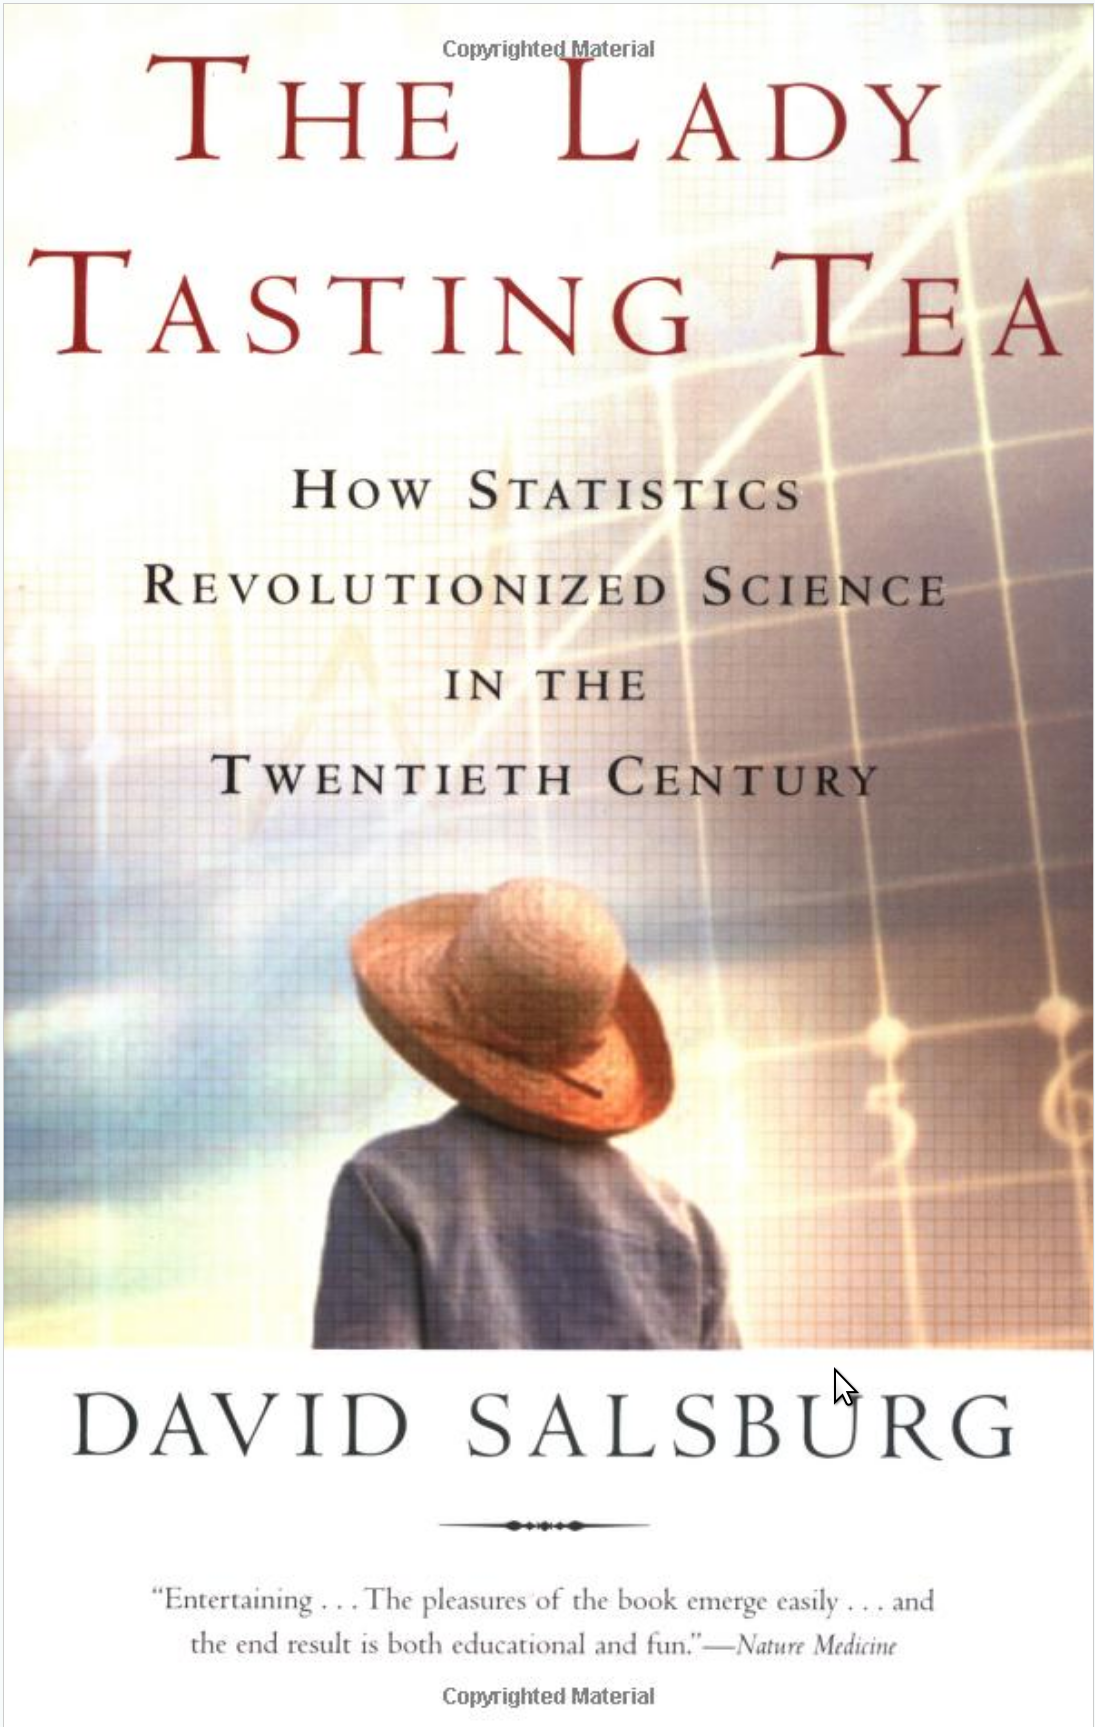
\includegraphics[width=0.25\textwidth]{media/book}
	\end{multicols}

	\note{Lets start with a bit of history. The idea that scientific measurements are best understood as reflecting underlying probabilities distributions is a relatively new idea.

It was a now famous thinker and scientist, Karl Pearson (of the Pearson correlation coefficient) who conceived the idea in late 18 hundreds.

He realized randomness was inherent part of nature and of scientific measure, and he formulated the idea that all measurments should be conceived of as coming from an underlying probability distributions.

In other words, the underlying truth is the distrubutions, and the measurements are just random reflections of this truth.  At the time, this was a revolutionary idea.}
\end{frame}

\begin{frame}[t]{The power of probability distributions}
	Distributions allow scientists to:
	\begin{itemize}
		\item Understand scientific measurement
		\item Predict the probability of specific data
		\item Test specific hypothesis (p-values)
		\item Produce generative models
		\item Better conceptual understanding data.
	\end{itemize}
	\note{And it was an idea that revolutized science.

	It allowed scientists to:
	\begin{itemize}
		\item Better understand their measurements.
		\item To make predictions about what data they should expect to observe.
		\item To test scientific hypotheses in a mathematically rigorous way.
		\item To build generative models of their data, and to test how well those models explain the observed measurments.
		\item And in general to have a better conceptual understanding of the data they generated.
	\end{itemize}
}
\end{frame}
%--- Next Frame ---%

\begin{frame}[t]{Estimating distributions from data}
	\begin{multicols}{2}
		Low-Dimensional:
		\begin{itemize}
			\item Great tools to fit and understand the underlying probability distribution of data.
		\end{itemize}
		\vfill\columnbreak
		High-Dimensional:
		\begin{itemize}
			\item In some cases, classical statistical tools are insufficient.
			\item Problematic for modern neuroscience: \begin{itemize}
				\item Thousands of electrodes.
				\item Millions of voxels.
			\end{itemize}
		\end{itemize}
	\end{multicols}
	\note{Since Pearson’s early work, scientists and statisticians have devised an enormous number of related tools.

For example they’ve defined many many distributions, and they’ve created tools for working with those distrubitons (calculating likelihoods and fitting them).

One class of tools aim to estimate the underlying distribution that generated an observed empirical measurment.

These tools are highly effective when data is low dimensional, but they are sometimes insufficient when data is high dimensional.}
\end{frame}
%--- Next Frame ---%

\begin{frame}[t]{How can we build statistical distributions for neuroscience datasets?}
	\movie[]{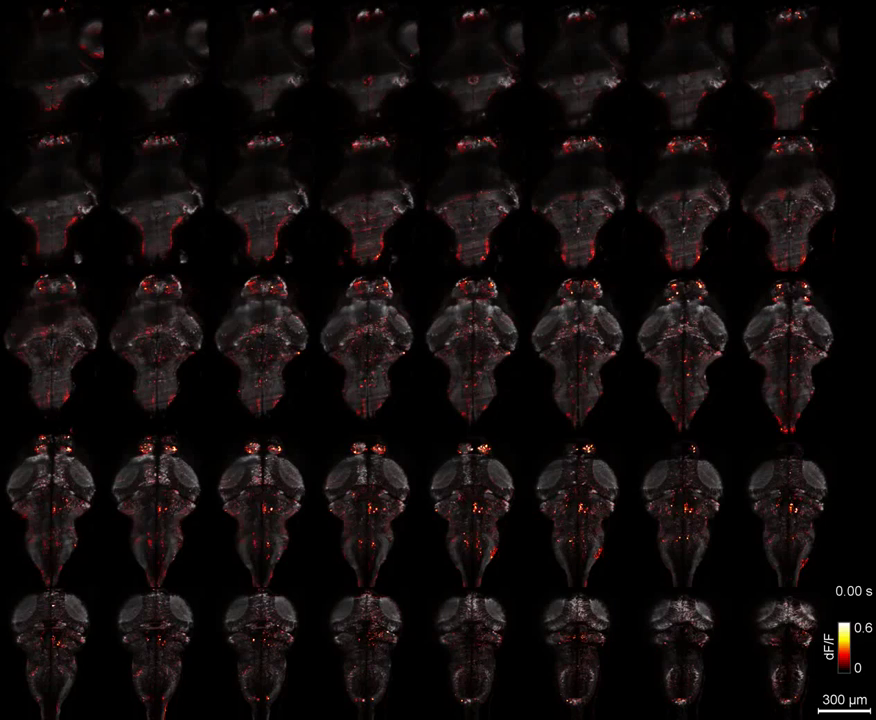
\includegraphics[width=0.7\textwidth,center]{media/zfish_first.png}}{media/zfish_imaging.mp4}
	\nakedfootnote{\url{https://www.youtube.com/watch?v=CXYp9xCUhe0}}
	\note{For example, consider whole brain imaging data from the zebrafish.  This data can have millions of dimensions, which makes estimating the understanding joint probability distribution difficult.  The number of possible states is enormous.  The voxels are not independent.  You can’t simply make a histogram or a heat-map.
			}
\end{frame}
%--- Next Frame ---%

\begin{frame}[t]{Variational Bayesian Methods}
	\note<1>{So this brings me to the topic I want to introduce today.  Variational Bayesian Methods.

Varitional Bayesian methods are powerful statistical approach for estimating the underlying probability distrution of high dimensional data.}
	\uncover<2>{
		Estimate the probability distribution of high-dimensional neural data.
		\begin{itemize}
			\item Compute the probability of observing a particular neural state.
			\item Sample neural states/trajectory from the estimate.
			\item Generate statistics / test hypotheses
			\item Estimate latent factors/states that drive the observations.
			\item Reduce dimensionality (with advantages over other methods, e.g. PCA, T-SNE)
		\end{itemize}
	}
	\note<2>{And this has several important possible uses in neuroscience.  By estimating the probability distrubiton of, say, whole brain calcium imaging data, one could: …}
\end{frame}
%--- Next Frame ---%

\section{\One}

\begin{frame}[t]{Approximating the area of a circle with Monte Carlo}
	\begin{center}
		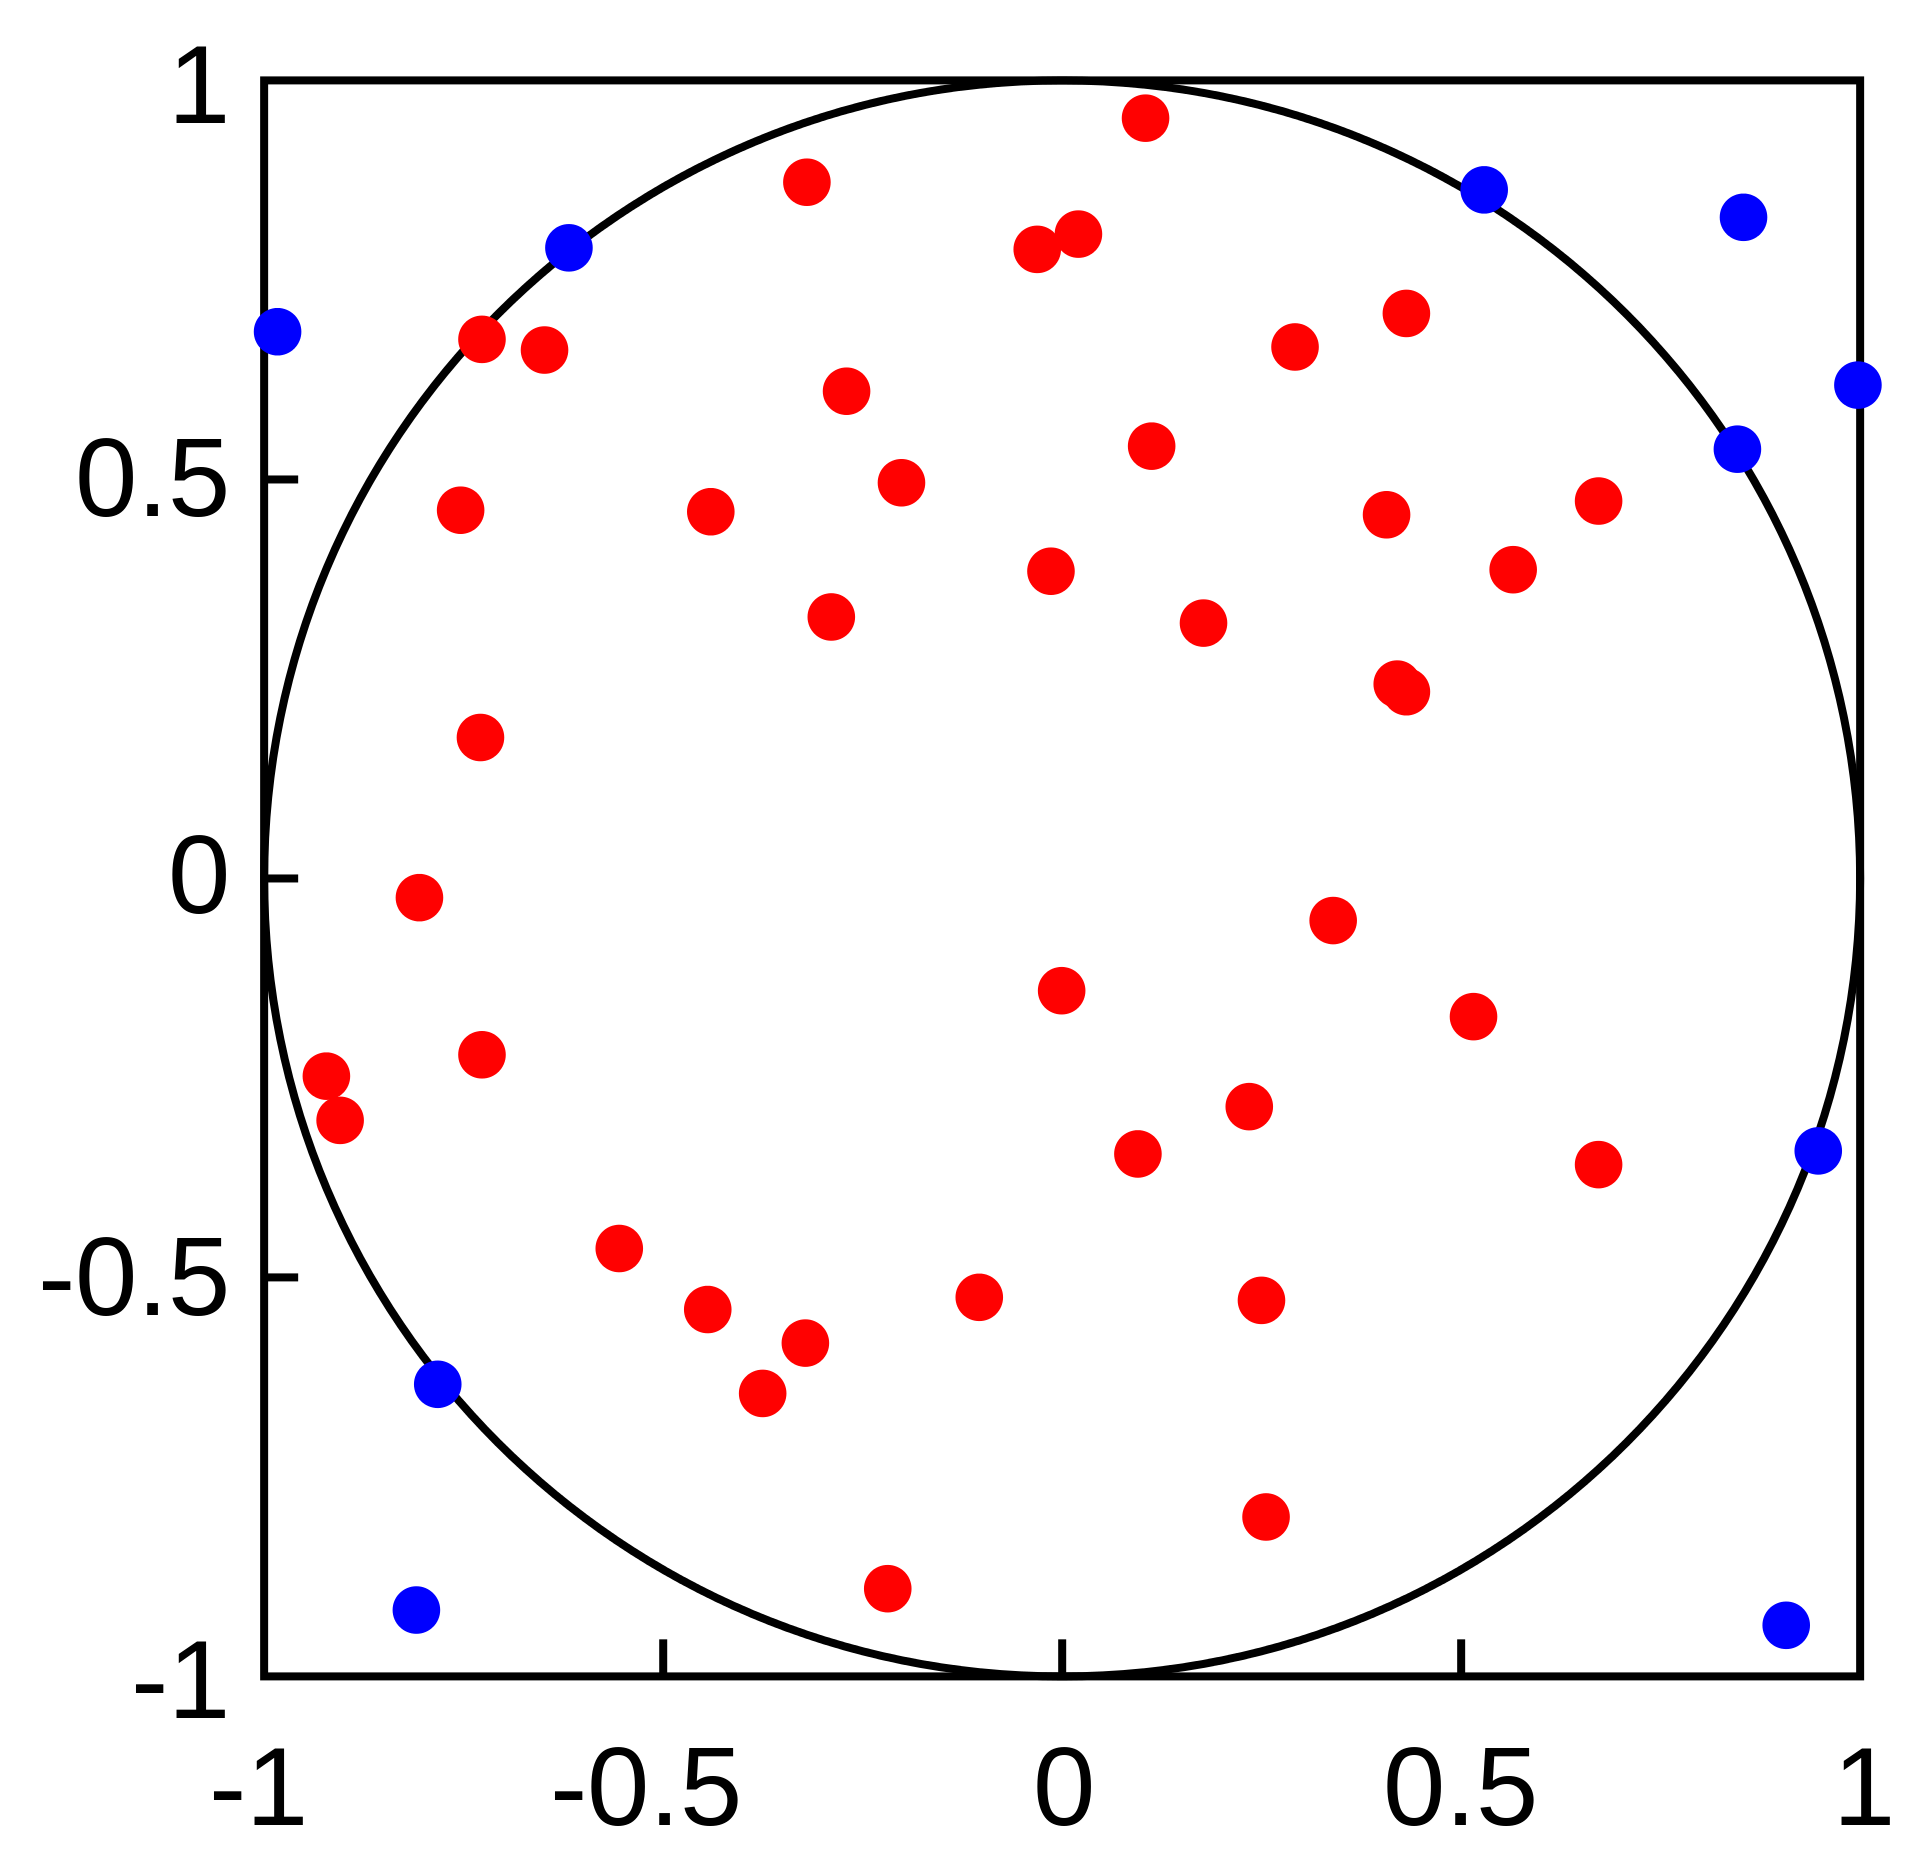
\includegraphics[height=0.75\textheight]{media/2d_monte_carlo}
		\linebreak
		40/50 samples in circle gives area of $4 * 0.8 = 3.2 \approx \pi$. $\sim 2\%$ error
	\end{center}
	\nakedfootnote{CCO 1.0, wikimedia, MonteCarloIntegrationCircle.svg}
\end{frame}

\begin{frame}[t]{Useful for analytically intractable integrals}
	\begin{center}
		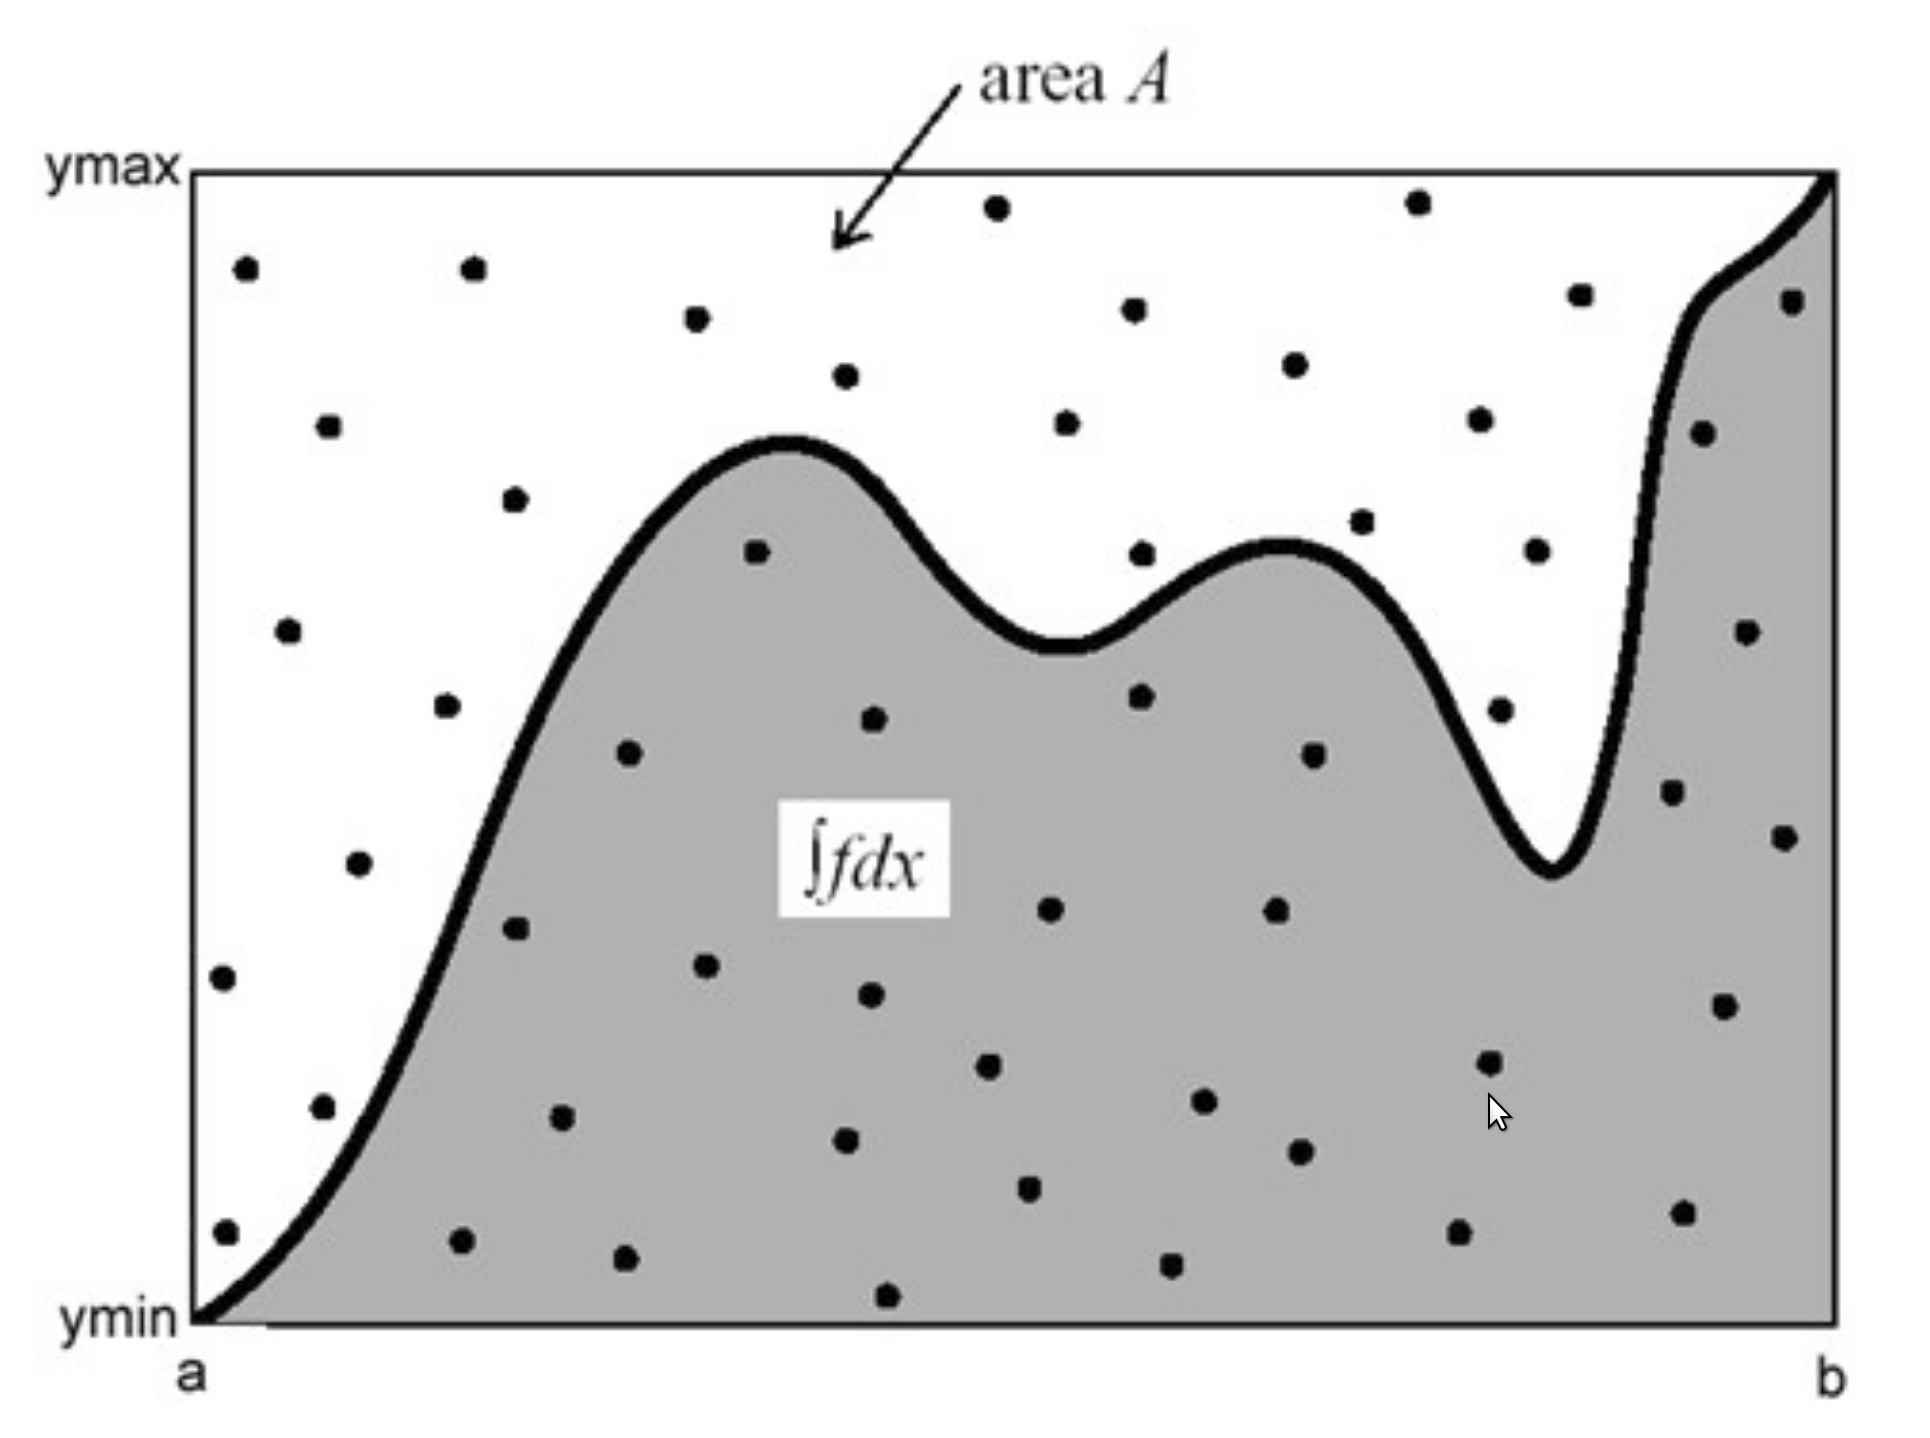
\includegraphics[height=0.75\textheight]{media/mc_integration}
	\end{center}
	\nakedfootnote{Robert Lin - Monte Carlo Integration }
\end{frame}

\begin{frame}[t]{Extension to unit hypercube}
	We can approximate a high-dimensional integral using a Monte Carlo approximation:
	\begin{align*}
		\int_0^1 \cdots \int_0^1 g(x_1,\dots,x_n) dx_1,\dots,dx_n
			\approx \frac{1}{N}\sum_{j=1}^N g(\bar{x}_j)
	\end{align*}
	where $\bar{x}_1,\dots,\bar{x}_N \sim \mathcal{U}(0,1)$ is the i\textsuperscript{th} random sample
\end{frame}


\begin{frame}[t]{Performance scales poorly with number of
	dimensions}
	\center
	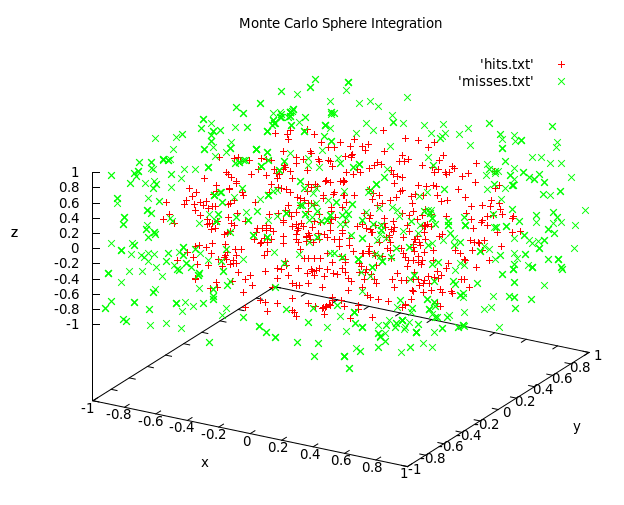
\includegraphics[height=0.8\textheight]{media/3d_monte_carlo}
	\linebreak
	1000 samples, estimate = 4.072, actual = 4.189, $\sim 3\%$ error
	\nakedfootnote{http://www2.hawaii.edu/~yuxian/phys305/a6/}
\end{frame}

\section{\Two}

\begin{frame}[t]{Alternate approach: Variational Bayes}{Variational auto-encoders and normalizing flows}
	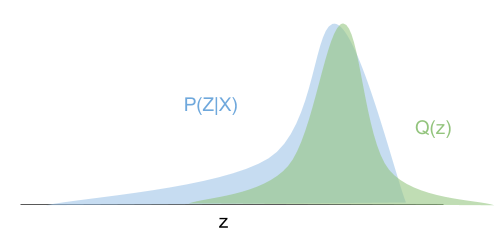
\includegraphics[height=0.5\textheight]{media/variational_gaussian}
	\includegraphics<2>[height=0.45\textheight]{media/normalizing_flow}
\end{frame}
%--- Next Frame ---%

\begin{frame}[t]{Variational auto-encoder}
	\vfill
	\center
	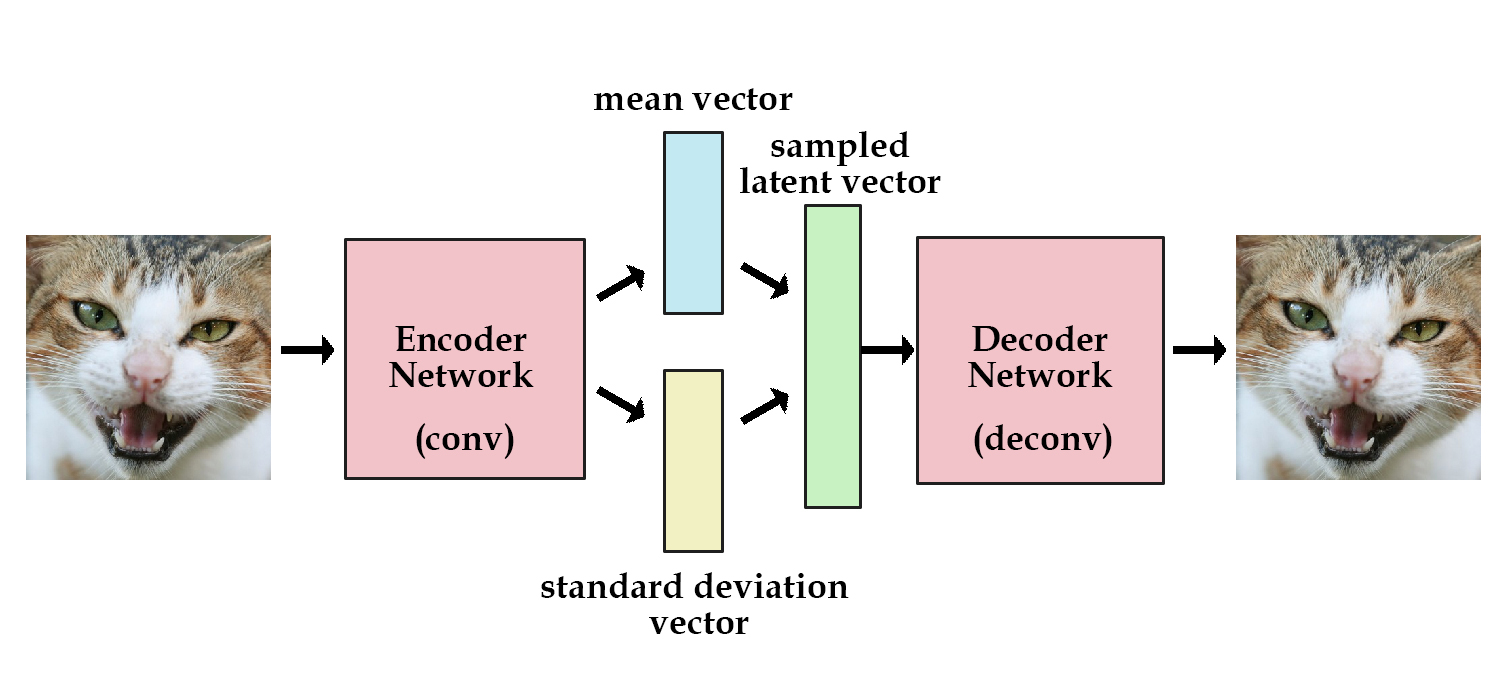
\includegraphics[width=\textwidth]{media/vae}
	Per-datapoint latent variable, $z_t$, which we construct by the \emph{encoder}, $e(x_t) = q_\phi(z_t|x_t)$, where q is parameterized by the variables $\phi$. We can reconstruct an approximation, $\hat{x}_t$, via a \emph{decoder}, $d(z_t) = p_\theta(x_t|z_t)$ with parameterizing variables $\theta$.
	\vfill
	\nakedfootnote{http://kvfrans.com/variational-autoencoders-explained/}
\end{frame}
%--- Next Frame ---%

\begin{frame}[t]{Derive lower bound $\rightarrow$ optimize!}
	Starting with the log probability of $x$, we derive (\ref{elbo}), the Evidence lower bound (ELBO):
	\begin{align}
	    \log p_\theta(x) &= \log \int_Z p_\theta(x,z) \\
	        &= \log \int_Z p_\theta(x,z) \frac{q_\phi(z|x)}{q_\phi(z|x)} \\
	        &= \log E_{q(z|x)}\left[\frac{p_\theta(x,z)}{q_\phi(z|x)}\right] \\
	        &\geq  E_{q(z|x)}\left[\log\frac{p_\theta(x,z)}{q_\phi(z|x)}\right] \label{jensen}\\
	        &= E_{q(z|x)}\left[\log p_\theta(x,z) \right] - H(q_\phi(z|x)) = L \label{elbo}
	\end{align}

	\note{Note that \ref{jensen} is true thanks to Jensen's inequality: $\varphi(E[X]) \geq E[\varphi(X)]$ for convex function $\varphi$. Intuitively, we want to improve our approximation of $p(x_t)$ by optimizing $\theta, \phi$ to maximize the ELBO.}
	\nakedfootnote{Kingma \& Welling 2013}
\end{frame}

\begin{frame}[t]{Understanding when the bound is tight}
	An alternate derivation gives insight for when this bound is tight:

	\begin{align}
	    \KL(q_\phi&(z|x)||p(z|x)) = \int_Z q_\phi(z|x) \log \frac{q_\phi(z|x)}{p_\theta(z|x)} \\
	        &= \int_Z q_\phi(z|x) \log \frac{q_\phi(z|x)p_\theta(x)}{p_\theta(x,z)} \\
	        &=  H(q_\phi(z|x)) + \log p_\theta(x) \int_Z q_\phi(z|x) - E_{q_\phi(z|x)}[\log p_\theta(x,z)] \\
	    L &= \log p_\theta(x) - \KL(q_\phi(z|x)||p_\theta(z|x))
	\end{align}
\end{frame}

% \section{\Three}

\begin{frame}[t]{Demo time!}
	\vfill
	\center
	\huge https://bit.ly/2LcEhow
	\vfill
\end{frame}

\begin{frame}[t]{Summary}
	\begin{itemize}
		\item \One \begin{itemize}
				\item
			\end{itemize}
		\item \Two \begin{itemize}
			\item
		\end{itemize}
		\item \Three \begin{itemize}
			\item
		\end{itemize}
	\end{itemize}
\end{frame}

\section{Discussion: Neuroscience applications}

\begin{frame}[t]{Example: LFADS}
	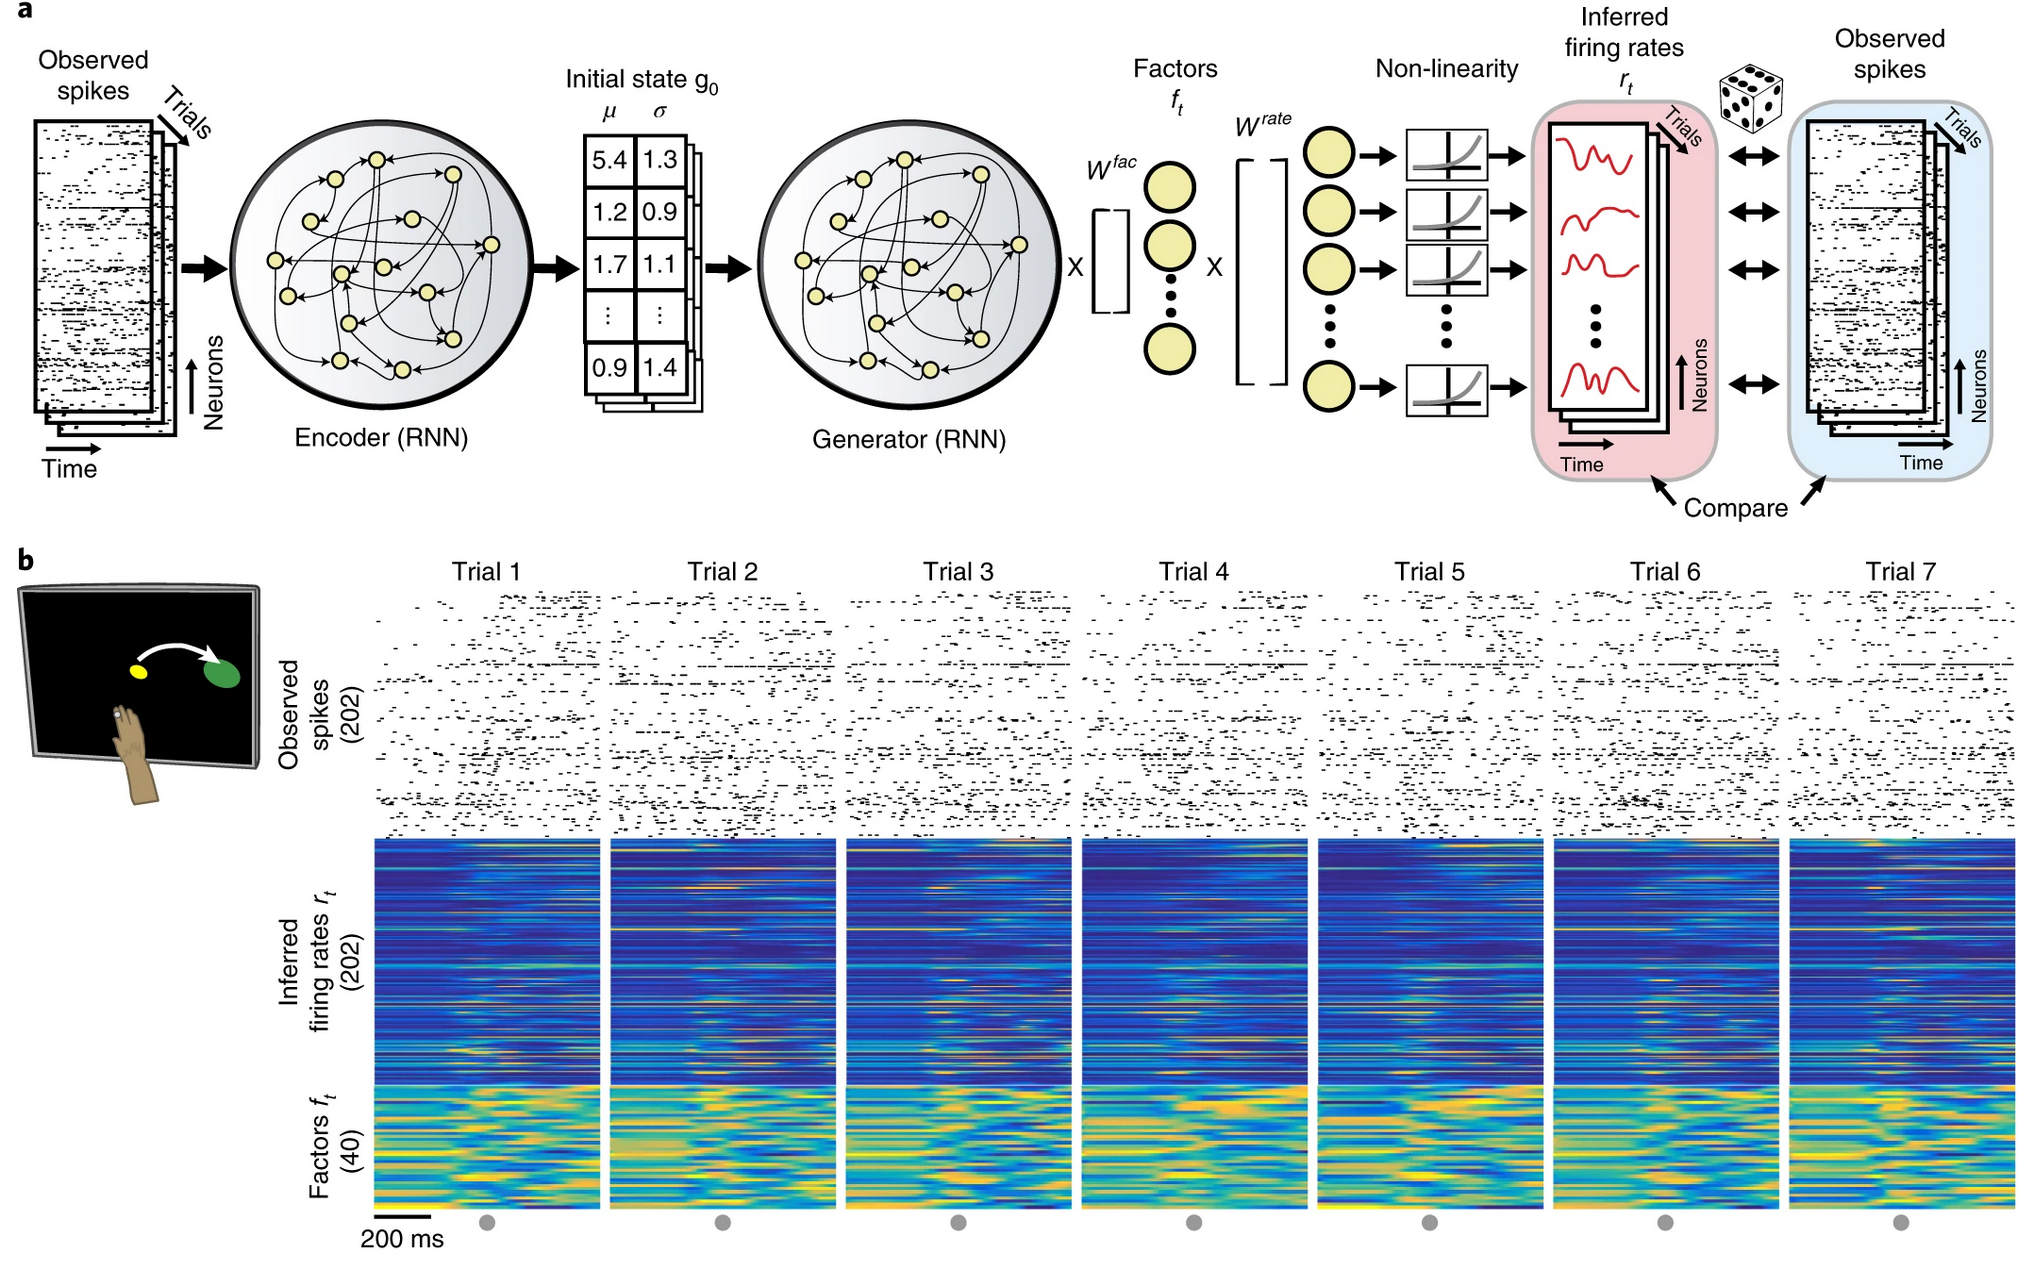
\includegraphics[width=\textwidth]{media/LFADS}
\end{frame}
%--- Next Frame ---%

\end{document}
